
%%%%%%%%%%%%%%%%%%%%%%%%%%%%%%%%%%%%%%%%%%%%%%%%%%%%%%%%%%%
\section{Experiment}\label{sec:expResults}
%%%%%%%%%%%%%%%%%%%%%%%%%%%%%%%%%%%%%%%%%%%%%%%%%%%%%%%%%%%



\subsection{Hardware system}


Our experiments are on centimeter-scale hardware systems called \emph{kilobots}.  These allows us to emulate a variety of dynamics, while enabling a high degree of control over robot function, the environment, and data collection. The kilobot, from \citet{Rubenstein2012,rubenstein2014programmable} is a low-cost robot designed for testing collective algorithms with large numbers of robots. It is available as an open source platform or commercially from~\citet{K-Team2015}.  Each robot is approximately 3 cm in diameter, 3 cm tall, and uses two vibration motors to move on a flat surface at speeds up to 1 cm/s.  Each robot has one ambient light sensor that is used to implement \emph{phototaxis},  moving towards a light source. 
In these experiments as shown in Fig.~\ref{fig:setup}, we used $n$=97 kilobots, a 1.5 m$\times$1.2 m whiteboard as the workspace, and eight 30W LED floodlights arranged 1.5 m above the plane of the table at the $\{N,NE,E,SE,S,SW,W,NW\}$ vertices of a 6 m square centered on the workspace. The lights were controlled using an Arduino Uno board connected to an 8-relay shield.  Above  the table, an overhead machine vision system tracks the position of the swarm.


\begin{figure}
\begin{center}
	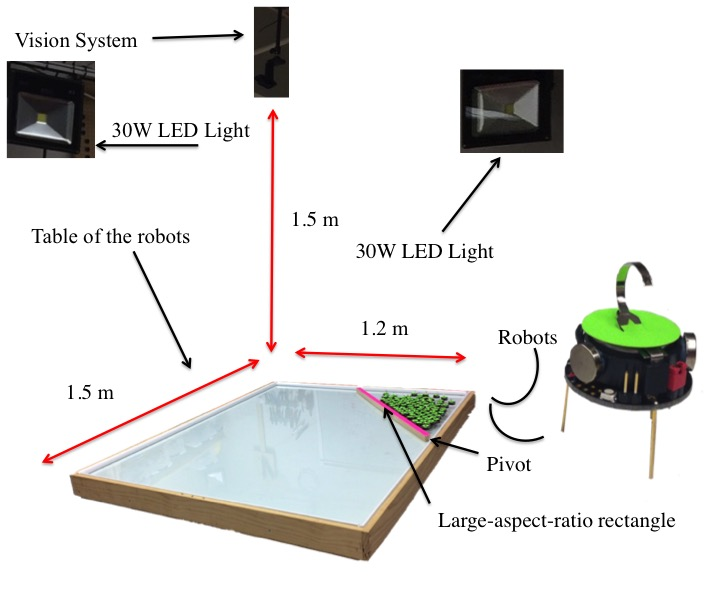
\includegraphics[width=\columnwidth]{SetUp.jpg}
\end{center}
\vspace{-1em}
\caption{\label{fig:setup}
Hardware platform:  table with 1.5$\times$1.2 m workspace, surrounded by eight remotely triggered 30W LED floodlights, with an overhead machine vision system.
}
\end{figure}

The walls of the hardware platform have almost infinite friction, due to a laser-cut, zigzag border and the three-legged design of the kilobots. When a kilobot is steered into the zigzag border, they pin themselves to the wall unless the global input directs them away from the wall.  This wall friction is sufficient to enable independent control of two kilobots, as shown in Fig.~\ref{fig:storyReal}.



\begin{figure*}[!htb]
\centering
\renewcommand{\figwid}{0.4\columnwidth}
{
\begin{overpic}[width =0.415\columnwidth]{twoR_1.pdf}\put(15,65){$t$  = 30 s}\end{overpic}\hspace{-.5em}
\begin{overpic}[width =\figwid]{twoR_2.jpg}\put(15,65){$t$  = 60 s}
\end{overpic}
\begin{overpic}[width =\figwid]{twoR_3.jpg}\put(15,65){$t$  = 90 s}
\end{overpic}
\begin{overpic}[width =\figwid]{twoR_4.jpg}\put(15,65){$t$  = 120 s}
\end{overpic}
\begin{overpic}[width =\figwid]{twoR_5.jpg}\put(15,65){$t$  = 150 s}
\end{overpic}}
\vspace{-1em}
\caption{\label{fig:storyReal}{Two robot positioning of two kilobot robots.  The boundary walls have nearly infinite friction, so the blue robot is stopped by the wall from $t = 30$s until the commanded input is directed away form the wall at $t=120$s, while the orange robot in free-space is unhindered.}
%\vspace{-2em}
}
\end{figure*}



To demonstrate covariance control $n$=97 robots were placed on the workspace and manually steered with a single light source, using friction with the boundary walls to vary the covariance from  -5000 to 10,000 pixel$^2$.  The resulting covariance is plotted in Fig.~\ref{fig:covExperiment}, along with snapshots of the swarm.




\begin{figure}
\begin{center}
	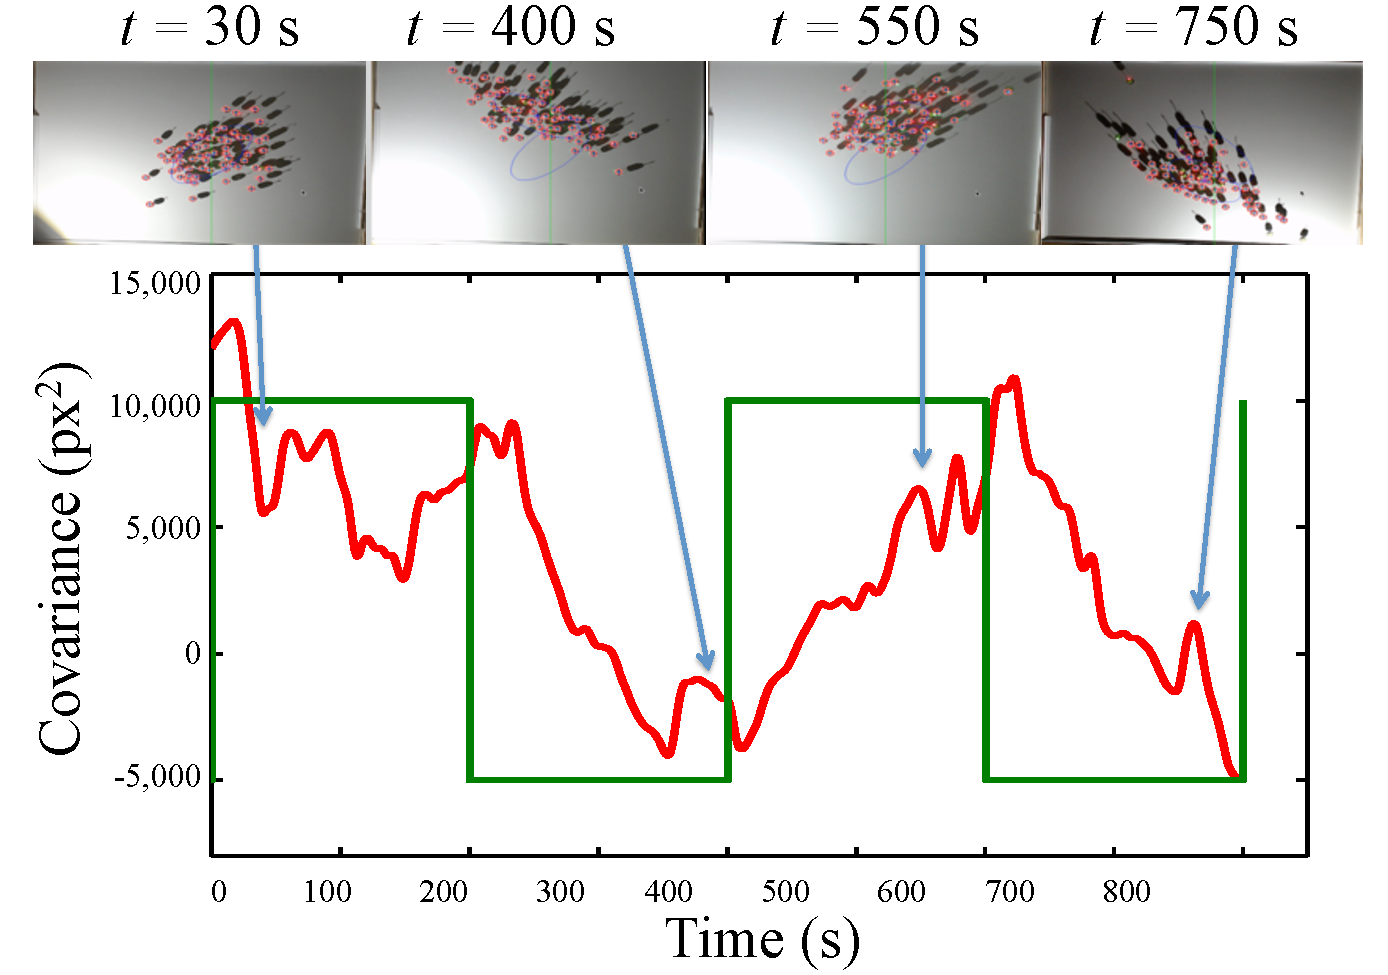
\includegraphics[width=\columnwidth]{experiment.pdf}
\end{center}
\vspace{-1em}
\caption{\label{fig:covExperiment}
Hardware demonstration steering 64 kilobot robots to desired covariance. The goal covariance is shown in green, the actual covariance in red. Frames above the plot show output from machine vision system and an overlaid covariance ellipse.
}
\end{figure}

